\subsection{Separately frozen extension: recovery, predictor comparison and map accuracy}\label{sec:extension}
The core evaluation was not modified. Because S2 stalled before any slowdown could act, we specified a post-evaluation extension, froze it on the pilot seeds 0--9 and evaluated it on fresh seeds 2000--2029. It makes three additions (Appendix~\ref{app:extension}).
\begin{enumerate}[label=\textbf{E\arabic*.},leftmargin=*]
\item \textbf{Recovery.} An online boat that has an empty queue and no committed exchange for one interval travels to a pre-agreed meeting cell at the grid centre. Travel is not a task claim. On contact, the boat finishes its current edge and accepts the new allocation. This is the simplest instance of the scheduled regrouping studied for communication-restricted exploration \cite{hollinger2010periodic,dasilva2024rendezvous,tan2024ir2}.
\item \textbf{Predictors.} Five further warning models share the S4 reservation action: an exponentially weighted residual (EWMA), a level/slope Kalman filter \cite{parasuraman2023rapid}, a Gilbert burst-state model, logistic regression and a 16-unit multilayer perceptron (MLP), the last two reflecting learned link-quality estimators \cite{cerar2021lqe,kanto2024lstm}. A non-deployable fade oracle that knows future fade states bounds the value of a perfect fade forecast. Margins and thresholds were selected by pilot F1. The learned models were fitted on seeds 0--6 and thresholded on 7--9.
\item \textbf{Map accuracy.} Every logged observation is replayed post hoc as a $10\times10$ swath of soundings over a synthetic analytic seabed of 14--37 m depth. Noise follows the IHO S-44 total vertical uncertainty $\mathrm{TVU}(d)=\sqrt{a^2+(bd)^2}$ for Order 1a ($a=0.5$ m, $b=0.013$) \cite{iho2020s44}, plus a 1 m horizontal offset per observation. Repeats are averaged and unobserved cells are filled by inverse-distance weighting.
\end{enumerate}
All 1980 extension logs passed the same reconstruction checks as the core.

\paragraph{Recovery changes the primary comparison but not the ranking of controls.} With recovery, every policy completed all 180 missions. S4-T was faster than S2 in all six conditions, by $108$--$175$ s ($-6.8\%$ to $-10.4\%$), and no interval included zero. The always-long queue S3 remained faster than S4-T by $13$--$28$ s ($0.9$--$1.9\%$), with every interval above zero. S1 remained fastest: online policies paid $70$--$179$ s (S3) and $204$--$363$ s (S2) for travel, rendezvous and allocation overhead (Table~\ref{tab:ext-contrasts}, Fig.~\ref{fig:ext-time}).

\paragraph{A better forecast did not buy a faster mission.} On held-out fixed-route replay, all deployable predictors except logistic regression reached F1 $0.185$--$0.193$, essentially the persistence value. Logistic regression reached only $0.106$, and the oracle reached $0.85$ (Table~\ref{tab:predictors}). In missions, no predictor beat S3: differences ranged from $0$ s (Gilbert and oracle, balanced progress) to $+77$ s (MLP). Even near-perfect fade warnings did not improve on always reserving a long queue. In this model the benefit comes from reservation capacity, not from forecast skill.

\paragraph{Computation is not the cost driver.} Per decision, the predictors ranged from 1 counted operation and 16 B of state (persistence) to 419 operations, 27 transcendental calls and 1.7 kB (MLP). Projected onto stated processor assumptions (Appendix~\ref{app:extension}), the worst case is the MLP on a Cortex-M4F with software binary64: at most $0.41$ ms, under $0.005\%$ of a 10 s exchange interval and under $1\%$ of 192 KiB SRAM. Each mission, by contrast, attempted $77$--$93$ kB of radio traffic. Predictor choice is therefore dominated by warning quality and by the communication and time it causes, not by arithmetic. This is an assumption-based projection, not a measured energy result.

\begin{figure}[htbp]\centering
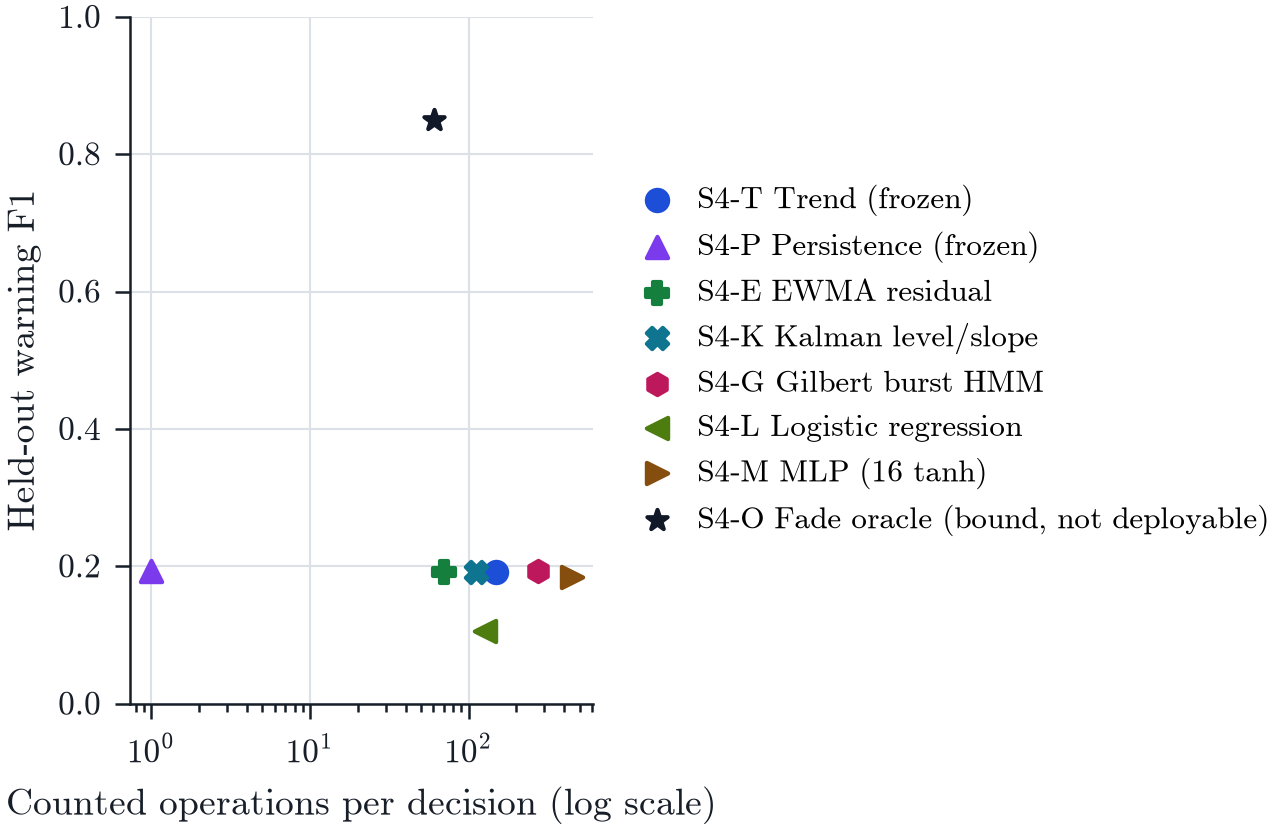
\includegraphics[width=.49\linewidth]{generated/extension/predictor-cost-quality.png}\hfill
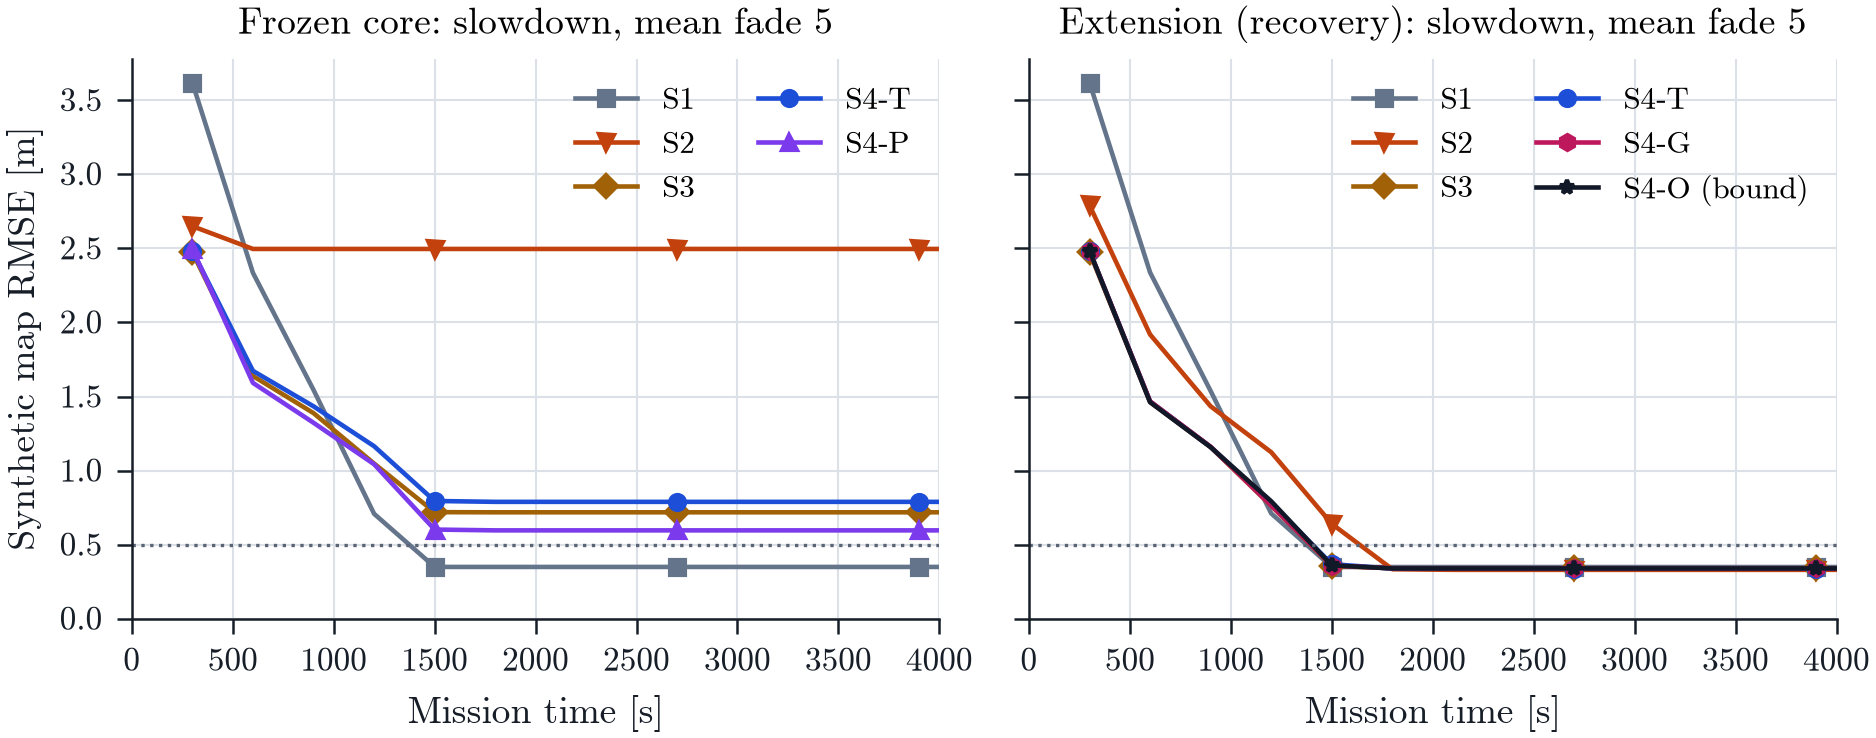
\includegraphics[width=.49\linewidth]{generated/extension/map-rmse-time.png}
\caption{Left: held-out warning F1 against counted operations per decision (log scale); $\times$ marks the non-deployable oracle. Right: mean synthetic map RMSE over time for the slowdown, $L=5$ condition; the dotted line is 0.5 m. Unfinished core S2 missions keep a large interpolation error.}\label{fig:ext-predictors-map}
\end{figure}

\paragraph{Coordination outcome and map accuracy differ.} In the frozen core, S2's final synthetic map RMSE was $2.50$ m, with only $34\%$ of soundings within the Order 1a TVU. The corresponding values were $0.53$--$0.60$ m and $85$--$87\%$ for S3/S4, and $0.35$ m and $92\%$ for S1. With recovery, all policies reached $0.33$--$0.35$ m and $92$--$93\%$. During the mission the ordering changes: at 900 s, online policies had RMSE $1.14$--$1.17$ m against $1.52$ m for S1, because distributed coverage interpolates better than a column-by-column sweep. Redundant passes slightly reduce final error (S2: 45 repeated cells, $0.332$ m). These values are synthetic and relative. They show that a policy's map quality depends on when the mission is stopped and on how much it repeats, not only on its completion time.
